\documentclass[11pt,a4paper,titlepage,draft]{article}
\usepackage[utf8]{inputenc}
\usepackage[greek]{babel}
\usepackage{amsmath}
\usepackage{amsfonts}
\usepackage{amssymb}
\usepackage{commath}
\usepackage{xcolor}
\usepackage{hyperref}
\usepackage[skins,theorems]{tcolorbox}
\usepackage{titlesec}
\usepackage{amsthm}
\usepackage{circuitikz}


\usetikzlibrary{arrows.meta}

\usepackage[left=2cm,right=2cm,top=2cm,bottom=2cm]{geometry}

\makeatletter
%\newcommand{\attnboxed}[1]{\textcolor{red}{\fbox{\normalcolor\m@th$\displaystyle#1$}}}
\makeatother
\tcbset{highlight math style={enhanced,colframe=red,colback=white,%
  arc=0pt,boxrule=1pt,shrink tight,boxsep=1.5mm,extrude by=0.5mm}}
\newcommand{\attnboxed}[1]{\tcbhighmath[colback=red!5!white,drop fuzzy shadow,arc=0mm]{#1}}
\titleformat{\section}{\bf\Large}{Κεφάλαιο \thesection}{1em}{}
\newtcolorbox{attnbox}[1]{colback=red!5!white,%
  colframe=red!75!black,fonttitle=\bfseries,title=#1}
\newtcolorbox{infobox}[1]{colback=blue!5!white,%
  colframe=blue!75!black,fonttitle=\bfseries,title=#1}


\title{Σημειώσεις Στατιστική \& Πιθανότητες}
\date{2016, Εαρινό εξάμηνο}
\author{Καναβούρας Κωνσταντίνος \\ \textlatin{\url{http://users.auth.gr/konkanant}}}



\begin{document}

\maketitle

%\tableofcontents

\newpage

\begin{itemize}
\item Γ. Ζιούτας Πιθανότητες
\item Δ. Κουγιουμτζής Στατιστική
\item Βιβλίο: Πιθανότητες και Στατιστική για Μηχανικούς, Γ. Ζιούτας
\end{itemize}

\paragraph{}

\begin{itemize}
\item Εξετάσεις: 8 μονάδες (τουλάχιστον 4/8 για να περάσει)
\item \textlatin{Test}: 2 μονάδες
\end{itemize}

\part{Πιθανότητες}

\section{}
\paragraph{Είδη φαινομένων}

\begin{enumerate}
\item \textbf{Αιτιοκρατικά} (καθοριστικά): Ξέρω το αποτέλεσμα του φαινομένου όταν γνωρίζω τα αίτια/τις προϋποθέσεις/το περιβάλλον του.
\item \textbf{Στοχαστικά}: Δεν μπορώ να προβλέψω το αποτέλεσμα, ακόμα και αν γνωρίζω τα παραπάνω.
\end{enumerate}
Μπορεί να υπάρχει και αβεβαιότητα λόγω μη ιδανικών μοντέλων πρόβλεψης. Ο μηχανικός πρέπει να γνωρίζει και να μπορεί να μετρά αυτήν την αβεβαιότητα.

\subsection{Πείραμα τύχης}
Στοχαστικό φαινόμενο που μπορούμε να δοκιμάσουμε όσες φορές θέλουμε, ακριβώς με τις ίδιες συνθήκες, και γνωρίζουμε όλα τα δυνατά αποτελέσματα, αν και δε γνωρίζουμε ακριβώς το αποτέλεσμα κάθε πειράματος.

\begin{itemize}
\item \(E\): Πείραμα τύχης (\textlatin{Experiment})
\item \(S\): \( \left\lbrace s_1,s_2, \dots , s_n \right\rbrace\) Δειγματοχώρος (\textlatin{Sample space})
\item \(s_i\): Δειγματοσημεία
\end{itemize}

\textit{π.χ.}
\begin{align*}
E_1 \qquad & S_1 = \left\lbrace 1,2,3,4,5,6 \right\rbrace \rightarrow \text{ ρίψη ζαριού}\\
E_2 \qquad & S_2 = \left\lbrace KKK, KK\Gamma , K\Gamma K, \Gamma K K, K \Gamma \Gamma, \Gamma \Gamma K, \Gamma \Gamma \Gamma \right\rbrace \rightarrow \text{ ρίψη κέρματος 3 φορές} \\
E_3 \qquad & S_3 = \left\lbrace 0,1,\dots,N \right\rbrace \rightarrow \text{ ελαττωματικά προϊόντα}\\
E_4 \qquad & S_4 = \left\lbrace 0,1,2,3\dots \right\rbrace \rightarrow \text{ αριθμός ατόμων που εκπέμπει ραδιενεργό υλικό}\\
E_5 \qquad & S_5 = \left\lbrace x | x \geq 0, x \in \mathbb R \right\rbrace \rightarrow \text{ χρόνος γενονότος}
\end{align*}

\paragraph{}
Υποσύνολα του δειγματικού χώρου, π.χ. \(A = \left\lbrace 4,5,6 \right\rbrace \subseteq S\) ονομάζονται γεγονότα. Συνήθως συμβολίζονται \(A,B,W,R\). Λέμε ότι ένα γεγονός πραγματοποιείται.

Το \(S\) είναι σίγουρο γεγονός.

το \(\left\lbrace \right\rbrace \subseteq S \) ονομάζεται αδύνατο γεγονός και συμβολίζεται \( \emptyset \).

\paragraph{}
\[S =  \left\lbrace s_1,s_2,\dots,s_n  \right\rbrace \]

Το δυναμοσύνολο \(S^*\) περιέχει όλα τα δυνατά υποσύνολα του \(S\):
\[S^* =  \left\lbrace  \left\lbrace  \right\rbrace,  \left\lbrace s_1 \right\rbrace, \left\lbrace s_2 \right\rbrace, \dots,  \left\lbrace s_n  \right\rbrace,  \left\lbrace s_1,s_2 \right\rbrace, \left\lbrace s_1,s_3 \right\rbrace, \dots,  \left\lbrace s_1,s_2,s_3 \right\rbrace \dots  \right\rbrace \]

Είναι:
\begin{align*}
(a+b)^n &= \binom{n}{0}a^nb^0 + \binom{n}{1}a^{n-1}b^1 + \binom{n}{2}a^{n-2}b^2 + \dots + \binom{n}{n} a^0b^n \\
(1+1)^n &= \binom{n}{0}\cdot 1 + \binom{n}{1}\cdot 1 + \binom{n}{2} \cdot 1+ \dots + \binom{n}{n} \cdot 1 \\
2^n &= \binom{n}{0} + \binom{n}{1} + \binom{n}{2} + \dots + \binom{n}{n}
\end{align*}
Παρατηρούμε ότι το \(S^*\) έχει \(2^n\) στοιχεία αν το \(S\) έχει \(n\).

\section*{Διαγράμματα \textlatin{Venn}}

% Definition of circles
\def\firstcircle{(0,0) circle (1.5cm)}
\def\secondcircle{(0:2cm) circle (1.5cm)}
\def\boundingbox{(-2cm,-2cm) rectangle (4cm,2cm)}
\colorlet{circle edge}{blue!50}
\colorlet{circle area}{blue!20}
\tikzset{filled/.style={fill=circle area, draw=circle edge, thick},
    outline/.style={draw=circle edge, thick}}
\setlength{\parskip}{5mm}


\begin{tikzpicture}
    \draw[outline] \firstcircle node {$A$};
    \draw[outline] \secondcircle node {$B$};
    \draw \boundingbox;
    \node[below right] at (current bounding box.south east) {$S$};
\end{tikzpicture}

\begin{tikzpicture}
    \draw[outline] (1,0) circle (1.5cm) node {$A=B$};
    \draw \boundingbox;
    \node[anchor=south] at (current bounding box.north) {Ισότητα};
\end{tikzpicture}

\begin{tikzpicture}
    \draw[outline] (1,0) circle (1.5cm) node {$A$};
    \draw[outline] (0.5,-0.75) circle (0.4cm) node {$B$};
    \draw \boundingbox;
    \node[anchor=south] at (current bounding box.north) {Περιεκτικότητα};
\end{tikzpicture}

\begin{tikzpicture}
    \draw[outline] (0,0) circle (1.5cm) node {$A$};
    \node at (2.5,-0.75) {$\overline{A}$};
    \draw \boundingbox;
    \node[anchor=south] at (current bounding box.north) {Συμπλήρωμα};
    \node[below right] at (current bounding box.south east) {$S$};
\end{tikzpicture}

\subsubsection{Πράξεις}
% Set A or B
\begin{tikzpicture}
    \draw[filled] \firstcircle node {$A$}
                  \secondcircle node {$B$};
    \draw \boundingbox;
    \node[anchor=south] at (current bounding box.north) {Ένωση $A \cup B$};
\end{tikzpicture}

% Set A and B
\begin{tikzpicture}
    \begin{scope}
        \clip \firstcircle;
        \fill[filled] \secondcircle;
    \end{scope}
    \draw[outline] \firstcircle node {$A$};
    \draw[outline] \secondcircle node {$B$};
    \draw \boundingbox;
    \node[anchor=south] at (current bounding box.north) {Τομή $A \cap B$};
\end{tikzpicture}


% Set A but not B
\begin{tikzpicture}
    \begin{scope}
        \clip \firstcircle;
        \draw[filled, even odd rule] \firstcircle node {$A$}
                                     \secondcircle;
    \end{scope}
    \draw[outline] \firstcircle
                   \secondcircle node {$B$};
    \draw \boundingbox;
    \node[anchor=south] at (current bounding box.north) {Διαφορά $A - B$};
\end{tikzpicture}


Παρατηρώ ότι:
\begin{align*}
(x-y)+y &= x \\
(A-B) \cup B &= A \cup B
\end{align*}

\subsubsection{Ιδιότητες}
\begin{itemize}
\item \(A \cup B = B \cup A\)
\item \(A \cup \left( B \cup \Gamma \right) = \left( A \cup B \right) \Gamma \)
\item \(A \cup \left( B \cap \Gamma \right) = \left( A \cup B \right) \cap \left( A \cup \Gamma \right) \)
\item \( \overline{A \cup B} = \overline{A} \cap \overline{B} \)
\end{itemize}

\subsubsection{}
\begin{align*}
S &=  \left\lbrace KK, K\Gamma, \Gamma K, \Gamma \Gamma \right\rbrace \\
A &=  \left\lbrace KK, K \Gamma, \Gamma K  \right\rbrace \leftarrow \text{ τουλάχιστον μία κεφαλή} \\
B &= \left\lbrace KK, \Gamma K  \right\rbrace \leftarrow \text{ κεφαλή στη 2η ρίψη} \\
\end{align*}
\begin{align*}
A\cup B &=  \left\lbrace KK, K \Gamma , \Gamma K  \right\rbrace \\
A\cap B &=  \left\lbrace KK,  \Gamma K  \right\rbrace \\
A-B &=  \left\lbrace K \Gamma  \right\rbrace
\end{align*}

\subsubsection{}
\[S,A,B, \Gamma \]
\begin{itemize}
\item Τουλάχιστον ένα από \(A,B, \Gamma \): \(A \cup B \cup  \Gamma \)
\item Μόνο ένα από τα \(Α,Β, \Gamma \): \(
\left( A - \left( B \cup \Gamma \right) \right) \cup
\left( B - \left( A \cup \Gamma \right) \right) \cup
\left( \Gamma  - \left( A \cup B \right) \right) =
\left( A \cap \overline{B} \cap \overline{C} \right) \cap
\left( \overline{A} \cap B \cap \overline{C} \right) \cap
\left( \overline{A} \cap \overline{B} \cap C \right)
\)
\item Ακριβώς δύο από τα \(A,B \Gamma \):
\(
\left(A \cap B - \Gamma \right) \cap
\left(A \cap \Gamma  - B \right) \cap
\left(B \cap  \Gamma - A \right)
\)
\item Το πολύ δύο από τα \(A,B, \Gamma\):
\(
\overline{A \cap B \cap \Gamma } = \overline{A} \cup \overline{B} \cup \overline{C}
\)
\end{itemize}

\paragraph{}
\textit{π.χ.}
\[A,B, \Gamma \]
Σε ένα παιχνίδι όπου κερδίζει ο παίκτης που πρώτος φέρνει κεφαλή, ποιο είναι το γεγονός να κερδίσει ο \(A\), αν \(A_i, B_i, \Gamma_i\) τα ενδεχόμενα στην \(i\)-οστή ρίψη να κερδίσει ένας παίκτης.
\[
WA = A_1 \cup \left( \overline{A_1} \cap \overline{B_2} \cap \overline{\Gamma_3} \cap A_4 \right) \cup \left( \overline{A_4} \cap \overline{B_5} \cap \overline{\Gamma_6} \cap A_7 \right) \cup \cdots
\]

\textit{\textlatin{H/W:}} Να βρεθούν τα \(WB, W \Gamma \).
\begin{align*}
WB &= \bar{A_1} \cap B_2 \cup 
\left( \overline{B_2} \cap \overline{C_3} \cap \overline{A_4} \cap B_5 \right) \cup
\left( \overline{B_5} \cap \overline{C_6} \cap \overline{A_7} \cap B_8 \right) \cup \cdots \\
WC &= \bar{A_1} \cap \overline{B_2} \cap C_3 \cup 
\left( \overline{C_3} \cap \overline{A_4} \cap \overline{B_5} \cap C_6 \right) \cup
\left( \overline{C_6} \cap \overline{A_7} \cap \overline{B_8} \cap C_9 \right) \cup \cdots \\
\end{align*}

\subsection{Πιθανότητα}
\(S, A\)
Πιθανότητα είναι να η βεβαιότητα να πραγματοποιηθεί ένα γεγονός.
\[ 0 \leq P(A) \leq 1 \]

\paragraph{}
\textit{π.χ.} Να βρεθεί η πιθανότητα να φέρει ζυγό αριθμό το ζάρι.

\begin{itemize}
\item \(S= \left\lbrace 1,2,3,4,5,6 \right\rbrace,\quad A =  \left\lbrace 2,4,6   \right\rbrace\). Άρα, αν χρησιμοποιήσουμε την κλασική μέθοδο για την εύρεση της πιθανότητας:
\[P(A) = \frac{N(A)}{N(S)} = \frac{3}{6} = 0,50\]
Η κλασική μέθοδος μπορεί να χρησιμοποιηθεί όταν είναι ισοπίθανα τα αποτελέσματα.

\item

\paragraph{Σχετική Συχνότητα}
Μπορώ να ρίξω πολλές ($N$) φορές το ζάρι:

\[ f(A) = \frac{N(A)}{N} \]
\[ P_A = \lim_{N \to \infty} \frac{N_A}{N} \]
\end{itemize}

\paragraph{}
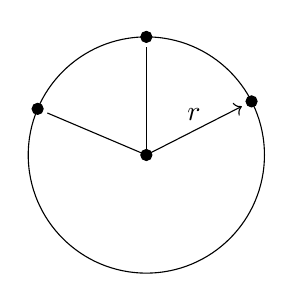
\begin{tikzpicture}
\draw (0,0) circle (1.5cm);
\filldraw[black] (0,0) circle (2pt);
\filldraw[black] (0,0) ++(157:1.5cm) circle[radius=2pt] node(A) {};
\filldraw[black] (0,0) ++(27:1.5cm) circle[radius=2pt] node(B) {};
\filldraw[black] (0,0) ++(90:1.5cm) circle[radius=2pt] node(C) {};


\draw[->] (0,0) -- (B) node[midway,above] {$r$};

\draw (0,0) -- (A);
\draw (0,0) -- (C);
\end{tikzpicture}
Ποια είναι η \(P ( AB \leq r ) \);
\begin{align*}
S&= \left\lbrace 1,2,3,\dots,360  \right\rbrace \\
AB &=\left\lbrace 1,2,3,\dots,120 \right\rbrace \rightarrow\text{ προκύπτει από γεωμετρία}
\end{align*}

\subsection{Αξιώματα \textlatin{Kolmogorov}}
\begin{enumerate}
\item \(0 \leq P(A) \leq 1\)
\item \( P(S) = 1\)
\item \( P(A \cup B) = P(A) + P(B) \)
\begin{tikzpicture}
    \draw[filled] (-0.25,0) circle(1cm) node {$A$}
                  (2.25,0) circle(1cm) node {$B$};
    \draw \boundingbox;
\end{tikzpicture}
\end{enumerate}

\paragraph{}
\(S= \left\lbrace \text{ΚΑ}, \text{SP},\text{MP},\text{KO} \right\rbrace\),
\(A=  \left\lbrace \text{KA}, \text{SP} \right\rbrace\). \(P(A) = \)?

\(P(A) = \frac{2}{4}\) (από κλασικό τρόπο), ή
\(P(\text{KA} \cup \text{SP}) = P(\text{KA})+P(\text{SP}) = \frac{1}{4} + \frac{1}{4}= \frac{1}{2}\), από το 3ο αξίωμα \textlatin{Kolmogorov}.

\subsection{}
\begin{enumerate}
\item \(P(\overline{A}) = 1-P(A)\)

\begin{proof}
\(P(\overline{A} \cup A) = P(S) \implies P(A) + P(\overline{A})=1\)
\end{proof}

\item \(P(\emptyset) = 0\)
\begin{proof}
\begin{align*}
P(\emptyset)&=1-P(\overline{\emptyset}) \\ &= 1-P(S) \\ &= 1-1 =0
\end{align*}
\end{proof}

\item \(P(A) \leq P(B)\)

\begin{tikzpicture}
    \draw[outline] (1,0) circle (1.5cm) node {$A$};
    \draw[outline] (0.5,0.75) circle (0.4cm) node {$B$};
    \draw \boundingbox;
\end{tikzpicture}
\begin{proof}
\begin{align*}
B = (B-A) \cup A \implies \\
P(B) &= P \left( (B-A) \cup A \right) \\
&= P(B-A) + P(A) \geq 0
\end{align*}
\end{proof}

\item \(P(A-B) = P(A) - P(A\cap B)\)

\begin{tikzpicture}
    \begin{scope}
        \clip \firstcircle;
        \draw[filled, even odd rule] \firstcircle node {$A$}
                                     \secondcircle;
    \end{scope}
    \draw[outline] \firstcircle
                   \secondcircle node {$B$};
    \draw \boundingbox;
\end{tikzpicture}

\begin{proof}
\begin{align*}
A = (A-B) \cup (A \cap B) \implies \\
P(A) &= P \left[ (A-B) \cup (A \cap B) \right] \\
&= P(A-B) + P(A \cap B)
\end{align*}
\end{proof}

\item \(P(A \cup B) = P(A) + P(B) - P(A \cap B) \)

% Set A and B
\begin{tikzpicture}
    \begin{scope}
        \clip \firstcircle;
        \fill[filled] \secondcircle;
    \end{scope}
    \draw[outline] \firstcircle node {$A$};
    \draw[outline] \secondcircle node {$B$};
    \draw \boundingbox;
    \node[anchor=south] at (current bounding box.north) {Τομή $A \cap B$};
\end{tikzpicture}


\begin{proof}
\begin{align*}
A \cup B = (A - B) \cup B \implies \\
P(A \cup B) &= P \left[ (A - B) \cup B \right] \\
&= P(A-B) + P(B) \\
&= P(A) -P(A \cap B) + P(B)
\end{align*}
\end{proof}

Μπορεί η παραπάνω σχέση να αποδειχθεί και για περισσότερα από δύο γεγονότα:
\[
P(A \cap B \cap \Gamma ) = P(A)+P(B)+P( \Gamma )-P(A\cap B) - P(A \cap \Gamma ) - P(B\cap\Gamma) + P(A \cap B \cap \Gamma )
\]
\end{enumerate}

\paragraph{}
\begin{circuitikz} \draw
(0,0) node[left] {$A$} to[closing switch=$\Delta_1$] (2,0) to [closing switch=$\Delta_2$] (4,0) node[right] {$B$};
\end{circuitikz}

\(P(\Delta_1)=0.5, \quad P(\Delta_1)=0.3, P(\Delta_1 \cap \Delta_3)=0.1\).\\
Τότε \(P(\Delta) = P(\Delta_1 \cup \Delta_2) = P(\Delta_1) + P(\Delta_2) - P(\Delta_1 \cap \Delta_2) = 0.7\).

\(S =  \left\lbrace \Delta_1\cap\Delta_2,\overline{\Delta_1}\cap\Delta_2,\Delta_1\cap\overline{\Delta_2},\overline{\Delta_1}\cap\overline{\Delta_2} \right\rbrace\)

\subsubsection{}
Για τρία σύνολα \(A,B, \Gamma \): Η πιθανότητα να συμβεί μόνο ένα από αυτά είναι: 
\begin{align*}
& P\left[
\left( A \cap \overline{B} \cap \overline{C} \right) \cap
\left( \overline{A} \cap B \cap \overline{C} \right) \cap
\left( \overline{A} \cap \overline{B} \cap C \right) \right] \\ &= 
P(A \cap \overline{B} \cap \overline{C}) + \dots \\ &= 
P\left[ A - (B \cap \Gamma )\right]
-P(A)-P \left[ A \cap (B \cap \Gamma ) \right] + \dots
\\ &= 
P(A) - P \left[ (A \cap B) \cup (A \cup \Gamma \right]+ \dots  \\ &= 
P(A) - \left( P(A \cap B) + P(A \cap \Gamma) - P(A\cap B\cap \Gamma ) \right)+ \dots  \\\ &=
P(A) - P(A \cap B) - P(A \cap \Gamma) + P(A \cap B \cap \Gamma)+ \dots
\end{align*}

\subsection{Δεσμευμένη πιθανότητα}
\(P(A\cap B) =\)?

\(P(A|B)\): η πιθανότητα να συμβεί το $A$ με την προϋπόθεση ότι $B$, ή η πιθανότητα να συμβεί το $A$, αν γνωρίζουμε ότι συμβαίνει το $B$, σε μια εκτέλεση του πειράματος.

\textit{π.χ.}

\begin{tikzpicture}
    \draw[outline] \firstcircle node {$A$};
    \draw[outline] \secondcircle node {$B$};
    \draw \boundingbox;
    \node at (-0.5,1) {$(3,3)$};
    \node at (-0.65,0.25) {$(3,1)$};
    \node at (-0.5,-1) {$(1,3)$};
    \node at (2,1) {$(2,6)$};
    \node at (3,0.85) {$(6,2)$};
    \node at (3,0.45) {$(2,5)$};
    \node at (3,0.15) {$(5,2)$};
    \node at (3,-0.15) {$(2,4)$};
    \node at (3,-0.45) {$(4,2)$};
    %TODO
\end{tikzpicture}

\(P(A) = \frac{5}{36},\ P(B) = \frac{11}{36}\) \\
Παρατηρώ ότι \(P(A)=\frac{2}{11} = \frac{\frac{N(A\cap B)}{n(s)}}{\frac{N(B)}{N(S)}}\).

Άρα, γενικά:
\[P \left( A | B \right) = \frac{P(A \cap B)}{P(B)} \]

Επομένως:
\begin{align*}
P(A \cap B) &= P(B)P(A|B) \\ &= P(A)P(B|A)
\end{align*}

\begin{itemize}
\item Αν \(A\cap B = \emptyset\), τότε \(P(A|B) = \emptyset\).
\item Αν \(A \subseteq B\), τότε \(P(B|A) = 1\).
\end{itemize}

\subsubsection{Πολλαπλαστιαστικός Κανόνας}
\begin{align*}
P(A_1 \cap A_2 \cap A_3 \cap \cdots \cap A_n) &= \\
&=P(A_1)P(A_2|A_1)P(A_3|A_1\cap A_2)\cdots P(A_n|A_1 \cap \cdots A_n)
\end{align*}

Μπορώ με τη χρήση του πολλαπλασιαστικού κανόνα να εντοπίσω την πιθανότητα 6 ρίψεις ζαριού να έχουν διαφορετικά νούμερα.
\begin{align*}
A_1 &= \left\lbrace \text{στην 1η ρίψη κάποιο νούμερο}  \right\rbrace \\
A_{i \geq 2} &= \left\lbrace \text{στην }i\text{ ρίψη νούμερο διάφορο από } A_{i-1},A_{i-2},\dots,A_1\text{ ρίψη}  \right\rbrace
\\\\
P(A_1 \cap A_2 \cap A_3 \cap A_4 \cap A_5 \cap A_6) &= P(A_1)P(A_2|A_1)P(A_3|A_1\cap A_2)\dots
\end{align*}

\end{document}